% !TeX root = main.tex

\section{Постановка задачи}

Задан объект
\[
\begin{cases}
\dot x_1=2x_2,\\
\dot x_2=8x_1+u
\end{cases}
\]
и критерий качества
\[
J=\int_0^4\left(x_1^2(\tau)+5x_1(\tau)x_2(\tau)
+7x_2^2(\tau)+3u^2(\tau)\right)\,d\tau
\]
Начальные и конечные условия:
\[
x_1(0)=x_2(0)=0,
\qquad x_1(4)=5,
\qquad x_2(4)=0
\]

Представим объект в матричной форме:
\[
\dot{\bm x}=A\bm x+\bm b u,
\qquad
A=\begin{pmatrix}0&2\\8&0\end{pmatrix},
\qquad
\bm b=\begin{pmatrix}0\\1\end{pmatrix}
\]
Подынтегральную функцию запишем в виде
\[
L(\bm x,u)=\bm x^{\mathsf T}Q\bm x+ru^2
\]
Для симметричной матрицы $Q$ имеем
\[
\bm x^{\mathsf T}Q\bm x
=q_{11}x_1^2+2q_{12}x_1x_2+q_{22}x_2^2
\]
Сопоставляя коэффициенты, получаем
\[
q_{11}=1,\qquad q_{12}=q_{21}=\frac52,\qquad q_{22}=7,
\]
\[
Q=\begin{pmatrix}1&\frac52\\[0.4ex]\frac52&7\end{pmatrix},
\qquad r=3
\]

\section{Необходимые условия оптимальности}

Введём сопряжённый вектор
$\bm\lambda=(\lambda_1,\lambda_2)^{\mathsf T}$
и составим гамильтониан в форме для задачи минимизации:
\[
H=\bm x^{\mathsf T}Q\bm x+ru^2
+\bm\lambda^{\mathsf T}(A\bm x+\bm b u)
\]

\[
H=x_1^2+5x_1x_2+7x_2^2+3u^2
+2\lambda_1x_2+\lambda_2(8x_1+u)
\]

Условие минимума по управлению:
\[
\frac{\partial H}{\partial u}=6u+\lambda_2=0,
\qquad
\frac{\partial^2 H}{\partial u^2}=6>0
\]
Отсюда
\[
\boxed{u^*=-\frac{\lambda_2}{6}}
\]

Сопряжённые уравнения определяются соотношением
\[
\dot{\bm\lambda}
=-\nabla_{\bm x}H
=-2Q\bm x-A^{\mathsf T}\bm\lambda
\]
В координатной форме:
\[
\begin{cases}
\dot\lambda_1=-2x_1-5x_2-8\lambda_2,\\
\dot\lambda_2=-5x_1-14x_2-2\lambda_1
\end{cases}
\]

\section{Краевая задача}

Подставляя найденное выражение для управления в уравнения объекта,
получаем совместную систему для состояний и сопряжённых переменных:
\[
\begin{cases}
    \dot x_1&=2x_2,\\
\dot x_2&=8x_1-\frac{\lambda_2}{6},\\
\dot\lambda_1&=-2x_1-5x_2-8\lambda_2,\\
\dot\lambda_2&=-5x_1-14x_2-2\lambda_1
\end{cases}
\]

\section{Аналитическое решение}

Сведём систему четырёх уравнений к одному уравнению для $x_1$.
Из уравнений объекта и соотношения $u^*=-\lambda_2/6$ находим
\[
 x_2=\frac{\dot x_1}{2},
\qquad
\lambda_2=6(8x_1-\dot x_2)=48x_1-3\ddot x_1
\]
Из второго сопряжённого уравнения выразим $\lambda_1$:
\[
\lambda_1=-\frac{\dot\lambda_2+5x_1+14x_2}{2}
=\frac{3x_1^{(3)}-55\dot x_1-5x_1}{2}
\]
Подставляя эти выражения в первое сопряжённое уравнение, получаем
\[
\frac{3x_1^{(4)}-55\ddot x_1-5\dot x_1}{2}
=-2x_1-\frac52\dot x_1-8(48x_1-3\ddot x_1)
\]
После приведения подобных слагаемых краевая задача принимает вид
\[
3x_1^{(4)}-103\ddot x_1+772x_1=0,
\]
\[
x_1(0)=\dot x_1(0)=0,
\qquad x_1(4)=5,\qquad \dot x_1(4)=0
\]

Для решения линейного уравнения с постоянными коэффициентами
используем подстановку $x_1=e^{st}$. Получаем характеристическое
уравнение $3s^4-103s^2+772=0$. Решая его как квадратное
относительно $s^2$, находим четыре различных действительных корня:
\[
s=\pm\alpha,\ \pm\beta,
\qquad
\alpha=\sqrt{\frac{103+\sqrt{1345}}6},
\qquad
\beta=\sqrt{\frac{103-\sqrt{1345}}6}
\]
Поэтому общее решение является линейной комбинацией
$e^{\alpha t}$, $e^{-\alpha t}$, $e^{\beta t}$ и $e^{-\beta t}$.
Объединим экспоненты с противоположными показателями с помощью
тождеств
\[
\cosh z=\frac{e^z+e^{-z}}2,
\qquad
\sinh z=\frac{e^z-e^{-z}}2
\]
Тогда то же решение можно записать в виде
\[
x_1(t)=A_1\cosh(\alpha t)+B_1\sinh(\alpha t)
+A_2\cosh(\beta t)+B_2\sinh(\beta t)
\]
Начальные условия $x_1(0)=\dot x_1(0)=0$ дают
\[
A_1+A_2=0,
\qquad \alpha B_1+\beta B_2=0
\]
Полагая $C=A_1$ и $D=\alpha B_1$, исключаем две постоянные:
\[
x_1^*(t)=C\bigl(\cosh(\alpha t)-\cosh(\beta t)\bigr)
+D\left(\frac{\sinh(\alpha t)}{\alpha}
-\frac{\sinh(\beta t)}{\beta}\right)
\]
Для определения постоянных $C,D$ используем конечные условия.
Так как $\dot x_1=2x_2$, условие $x_2(4)=0$ равносильно
$\dot x_1(4)=0$. Подставляя $t=4$ в выражения для
$x_1^*(t)$ и его производной, получаем систему
\[
\begin{cases}
C\bigl(\cosh(4\alpha)-\cosh(4\beta)\bigr)
+D\left(\dfrac{\sinh(4\alpha)}{\alpha}
-\dfrac{\sinh(4\beta)}{\beta}\right)=5,\\[6pt]
C\bigl(\alpha\sinh(4\alpha)-\beta\sinh(4\beta)\bigr)
+D\bigl(\cosh(4\alpha)-\cosh(4\beta)\bigr)=0
\end{cases}
\]
Обозначим коэффициенты этой системы:
\[
\begin{aligned}
h&=\cosh(4\alpha)-\cosh(4\beta),\\
p&=\frac{\sinh(4\alpha)}{\alpha}
-\frac{\sinh(4\beta)}{\beta},\\
q&=\alpha\sinh(4\alpha)-\beta\sinh(4\beta)
\end{aligned}
\]
Тогда система принимает вид
\[
\begin{cases}
hC+pD=5,\\
qC+hD=0
\end{cases}
\]
Её определитель равен
\[
\Delta=\begin{vmatrix}h&p\\q&h\end{vmatrix}=h^2-pq
\]
По правилу Крамера находим
\[
C=\frac{\begin{vmatrix}5&p\\0&h\end{vmatrix}}{\Delta}
=\frac{5h}{\Delta},
\qquad
D=\frac{\begin{vmatrix}h&5\\q&0\end{vmatrix}}{\Delta}
=-\frac{5q}{\Delta}
\]
Возвращаясь к исходным обозначениям, получаем
\[
C=\frac{5\bigl(\cosh(4\alpha)-\cosh(4\beta)\bigr)}{\Delta},
\qquad
D=-\frac{5\bigl(\alpha\sinh(4\alpha)-\beta\sinh(4\beta)\bigr)}{\Delta},
\]
где после раскрытия произведений в $h^2-pq$ имеем
\[
\begin{aligned}
\Delta={}&\cosh^2(4\alpha)+\cosh^2(4\beta)
-2\cosh(4\alpha)\cosh(4\beta)\\
&-\sinh^2(4\alpha)-\sinh^2(4\beta)
+\left(\frac\alpha\beta+\frac\beta\alpha\right)
\sinh(4\alpha)\sinh(4\beta)
\end{aligned}
\]
Используя тождество $\cosh^2z-\sinh^2z=1$, окончательно получаем
\[
\Delta=\frac{\alpha^2+\beta^2}{\alpha\beta}
\sinh(4\alpha)\sinh(4\beta)
-2\cosh(4\alpha)\cosh(4\beta)+2
\]
Для рассматриваемой задачи $\Delta\approx5{,}03805\cdot10^{12}\ne0$,
поэтому постоянные определены однозначно:
\[
\begin{aligned}
\alpha&\approx4{,}824835776856,&
\beta&\approx3{,}324799702193,\\
C&\approx1{,}191785974520\cdot10^{-4},&
D&\approx-5{,}754613296777\cdot10^{-4}
\end{aligned}
\]

Вторая координата:
\[
\begin{aligned}
x_2^*(t)={}&\frac C2\bigl(\alpha\sinh(\alpha t)
-\beta\sinh(\beta t)\bigr)\\
&+\frac D2\bigl(\cosh(\alpha t)-\cosh(\beta t)\bigr)
\end{aligned}
\]
Оптимальное управление $u^*=\ddot x_1^*/2-8x_1^*$ имеет вид
\[
\boxed{
\begin{aligned}
u^*(t)={}&C\left[\left(\frac{\alpha^2}{2}-8\right)\cosh(\alpha t)
-\left(\frac{\beta^2}{2}-8\right)\cosh(\beta t)\right]\\
&+D\left[\left(\frac\alpha2-\frac8\alpha\right)\sinh(\alpha t)
-\left(\frac\beta2-\frac8\beta\right)\sinh(\beta t)\right]
\end{aligned}}
\]

После подстановки численных значений:
\[
\boxed{
\begin{aligned}
u^*(t)\approx{}&-1{,}675250277027\cdot10^{-7}e^{4{,}824835776856t}
+4{,}339204303317\cdot10^{-4}e^{-4{,}824835776856t}\\
&-6{,}664699353563\cdot10^{-5}e^{3{,}324799702193t}
+3{,}613582018123\cdot10^{-4}e^{-3{,}324799702193t}
\end{aligned}}
\]

Найденное управление является единственным глобальным минимумом
среди управлений, удовлетворяющих заданным краевым условиям.
Действительно, $q_{11}=1>0$, $\det Q=3/4>0$ и $r=3>0$,
поэтому подынтегральная функция строго выпукла по состоянию
и управлению, а динамика и краевые ограничения линейны.
Следовательно, выполненные условия стационарности достаточны
для глобального минимума.

\section{Результаты моделирования}

Моделирование проведено в Simulink на интервале $0\le t\le4$~с
с фиксированным шагом $10^{-4}$~с. В модели \texttt{lab1.slx}
блок MATLAB Function формирует найденное управление $u^*(t)$,
а блок State-Space реализует уравнения объекта с матрицами
$A$, $\bm b$ и нулевыми начальными условиями.
Состояние и управление сохраняются в переменных
\texttt{out.y} и \texttt{out.u}. В файле \texttt{lab2.mlx}
критерий вычисляется методом трапеций как накопленный интеграл
\[
J(t)=\int_0^t\left(x_1^2(\tau)+5x_1(\tau)x_2(\tau)
+7x_2^2(\tau)+3u^2(\tau)\right)\,d\tau
\]
Первая координата достигает заданного значения $x_1(4)=5$,
а вторая к концу интервала возвращается к нулю. При проверочном
запуске получены $x_1(4)\approx4{,}9999999984$ и
$|x_2(4)|<4\cdot10^{-9}$.
Основное изменение состояния происходит в конце интервала:
сначала $x_2$ возрастает, обеспечивая рост $x_1$, затем
уменьшается до нуля под действием отрицательного управления.
Такое поведение согласуется с уравнением $\dot x_1=2x_2$.
Максимум $x_2\approx3{,}64$ достигается при $t\approx3{,}75$~с;
в конце интервала $u^*(4)\approx-80{,}10$.
Накопленный критерий не убывает, поскольку подынтегральная
квадратичная форма положительно определена. Его основная
часть набирается на заключительном участке, где велики
состояние объекта и модуль управления. По результатам расчёта
\[
\boxed{J^*=J(4)\approx2482{,}50}
\]

Траектории состояния, управление и критерий представлены
на рисунке~\ref{fig:optimal-response}.

\clearpage
\begin{figure}[H]
    \centering
    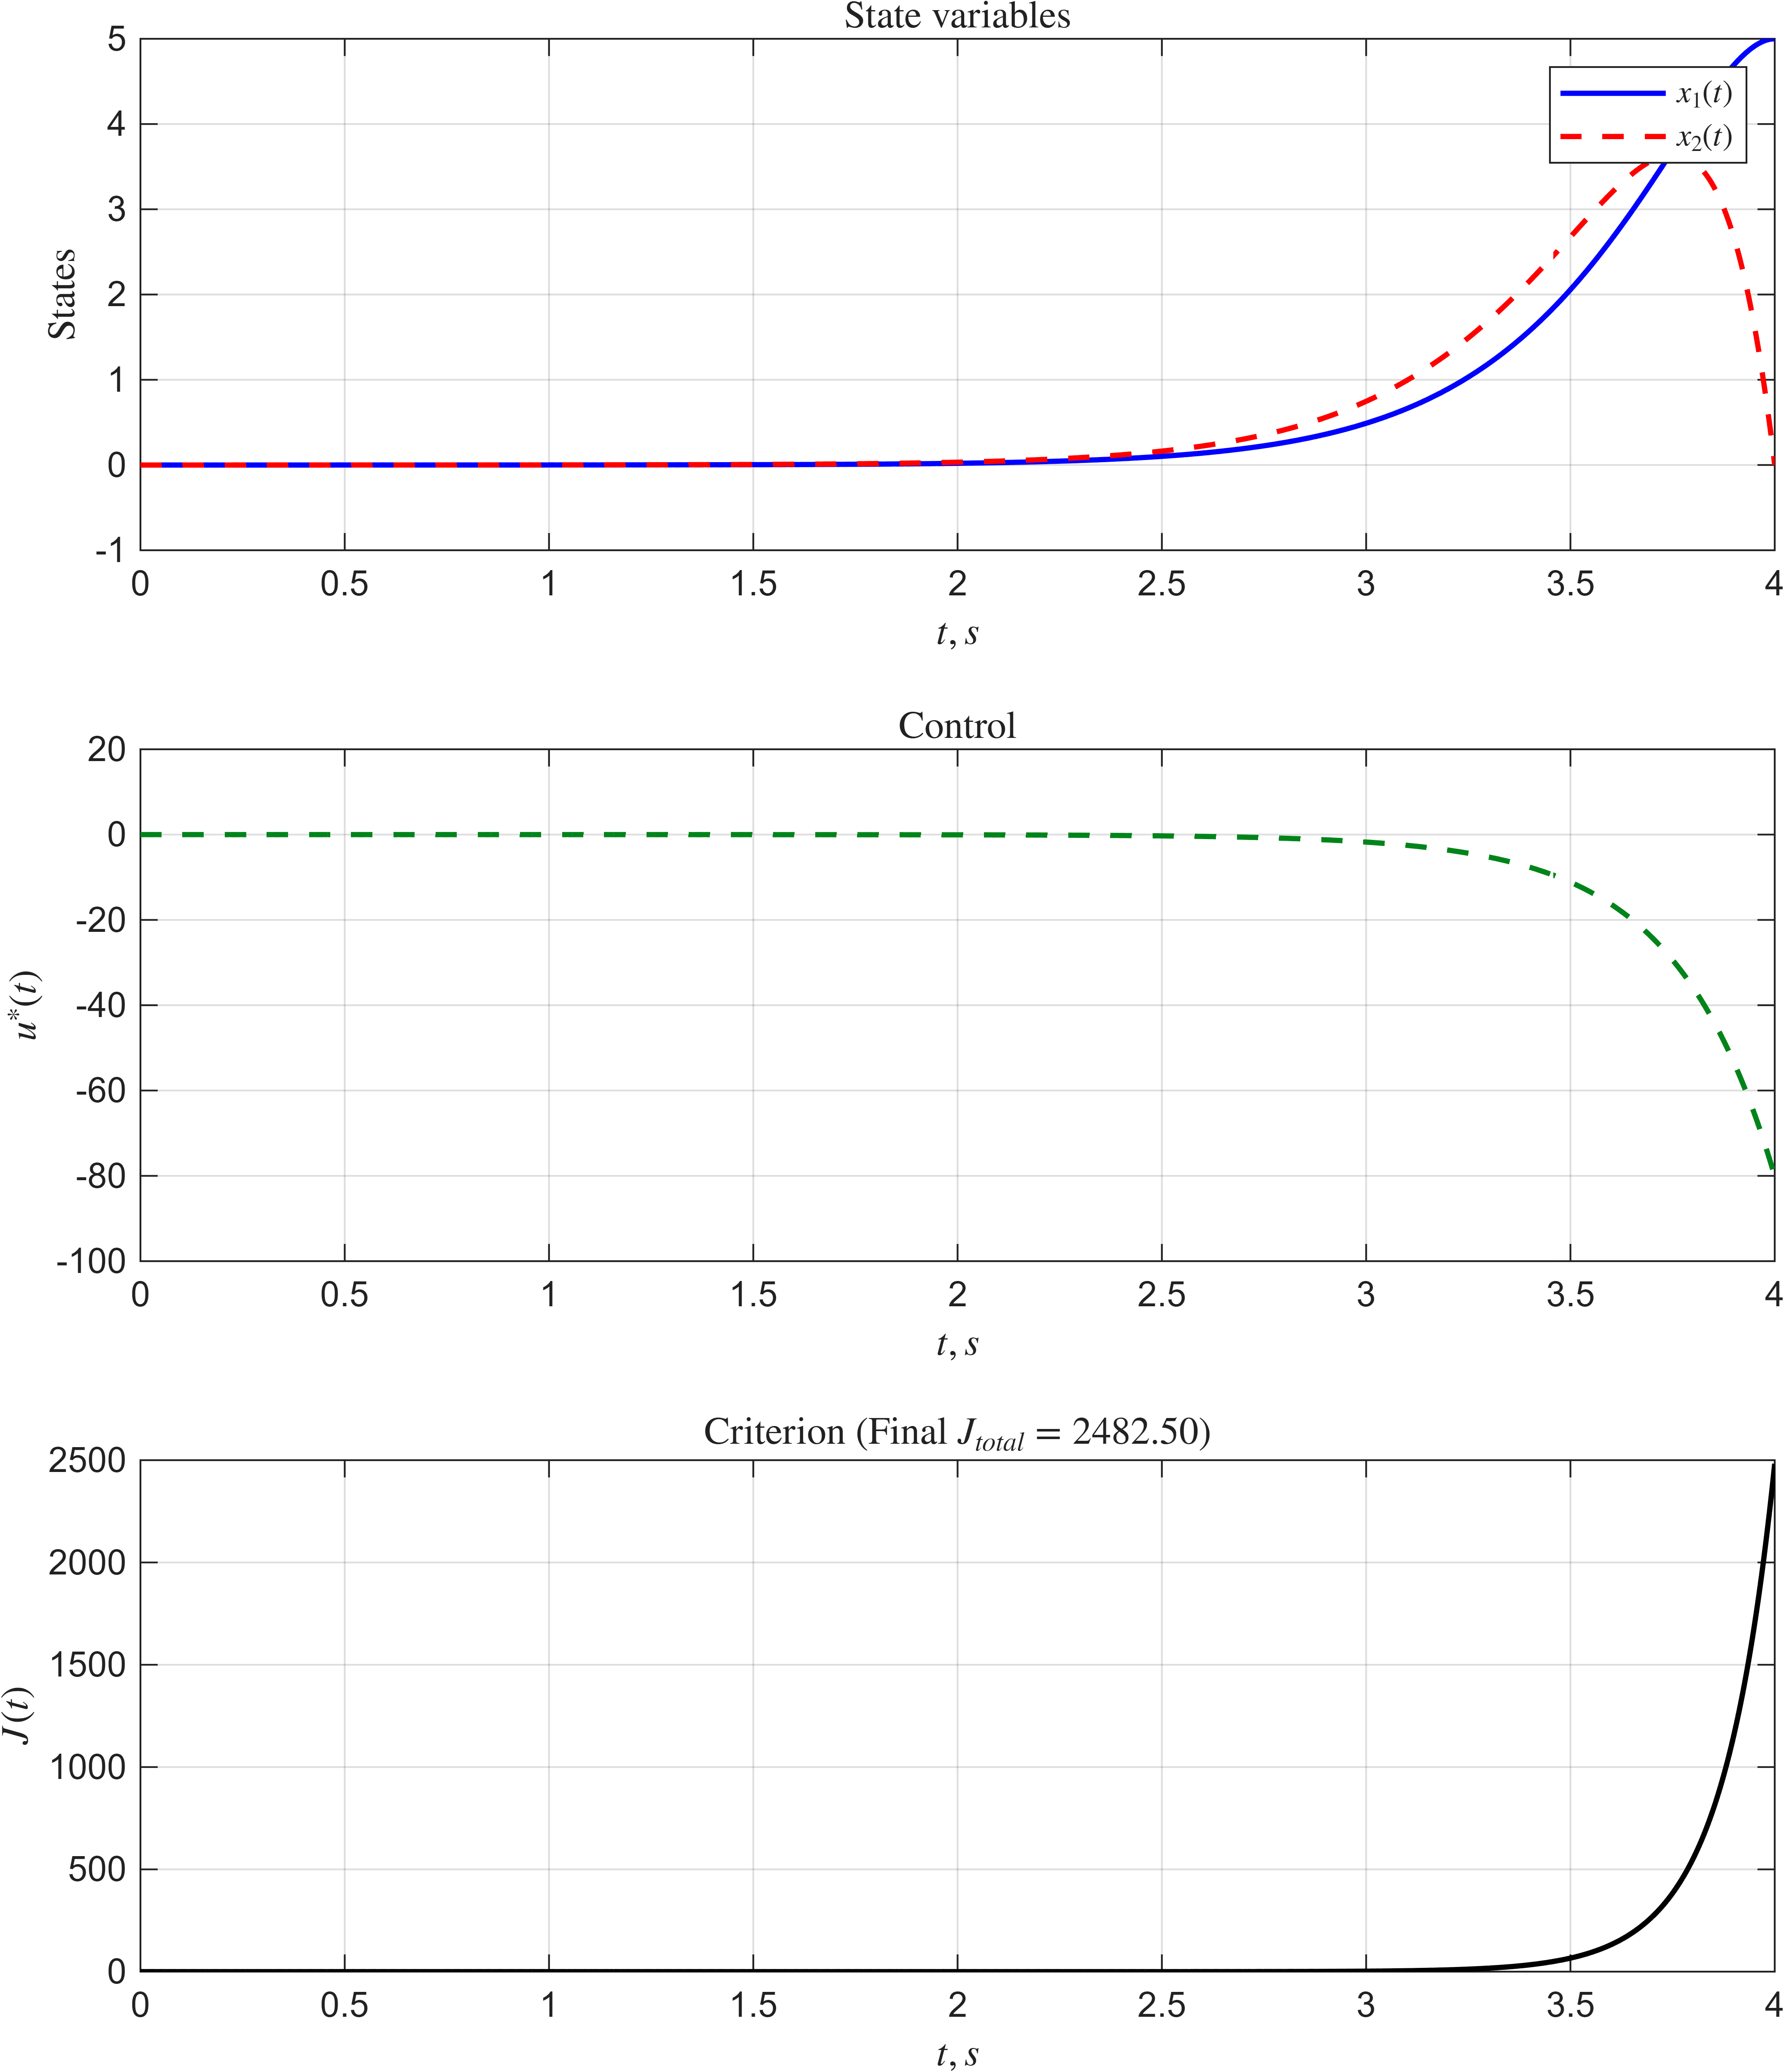
\includegraphics[width=\linewidth,height=0.78\textheight,keepaspectratio]{lab1_plots.png}
    \caption{Состояние объекта, оптимальное управление и накопленный критерий}
    \label{fig:optimal-response}
\end{figure}

\clearpage
Исследуем влияние отклонения общего множителя управления:
\[
u(t)=u_cu^*(t),
\qquad
u_c\in\left\{\frac45,\frac{14}{15},\frac{16}{15},\frac65\right\}
\]
Эти значения получены в MATLAB командой
\texttt{linspace(0.8, 1.2, 4)}; в легендах рисунка
они округлены до $0{,}80$, $0{,}93$, $1{,}07$ и $1{,}20$.
Параметры объекта и критерий качества при этом не изменялись.
Результаты приведены на рисунке~\ref{fig:control-sensitivity}.

Объект линеен, а начальное состояние равно нулю. Поэтому
масштабирование управления в $u_c$ раз масштабирует всё
состояние в столько же раз:
\[
\bm x(t;u_c)=u_c\bm x^*(t)
\]
Отсюда для конечного состояния и квадратичного критерия получаем
\[
x_1(4;u_c)=5u_c,
\qquad x_2(4;u_c)=0,
\qquad J(4;u_c)=u_c^2J^*
\]
Расчётные значения приведены в таблице~\ref{tab:control-sensitivity}.

\begin{table}[H]
    \centering
    \caption{Критерий качества и конечное состояние при отклонении множителя управления}
    \label{tab:control-sensitivity}
    \begin{tabular}{ccccc}
        \toprule
        $u_c$ & $x_1(4)$ & $x_1(4)-5$ & $x_2(4)$ & $J(4)$ \\
        \midrule
        $0{,}8$ & $4{,}000$ & $-1{,}000$ & $\approx0$ & $1588{,}80$ \\
        $14/15$ & $4{,}667$ & $-0{,}333$ & $\approx0$ & $2162{,}53$ \\
        $1$ & $5{,}000$ & $0$ & $\approx0$ & $2482{,}50$ \\
        $16/15$ & $5{,}333$ & $0{,}333$ & $\approx0$ & $2824{,}53$ \\
        $1{,}2$ & $6{,}000$ & $1{,}000$ & $\approx0$ & $3574{,}80$ \\
        \bottomrule
    \end{tabular}
\end{table}

При уменьшении $u_c$ критерий уменьшается, но одновременно
нарушается условие $x_1(4)=5$. Поэтому значения $J(4)<J^*$
при $u_c<1$ не противоречат оптимальности найденного управления:
соответствующие траектории не являются допустимыми для исходной
задачи с фиксированным конечным состоянием.
При $u_c>1$ наблюдаются превышение заданной первой координаты
и увеличение критерия. В рассматриваемом семействе управлений
оба конечных условия выполняются только при $u_c=1$.

\clearpage
\begin{figure}[H]
    \centering
    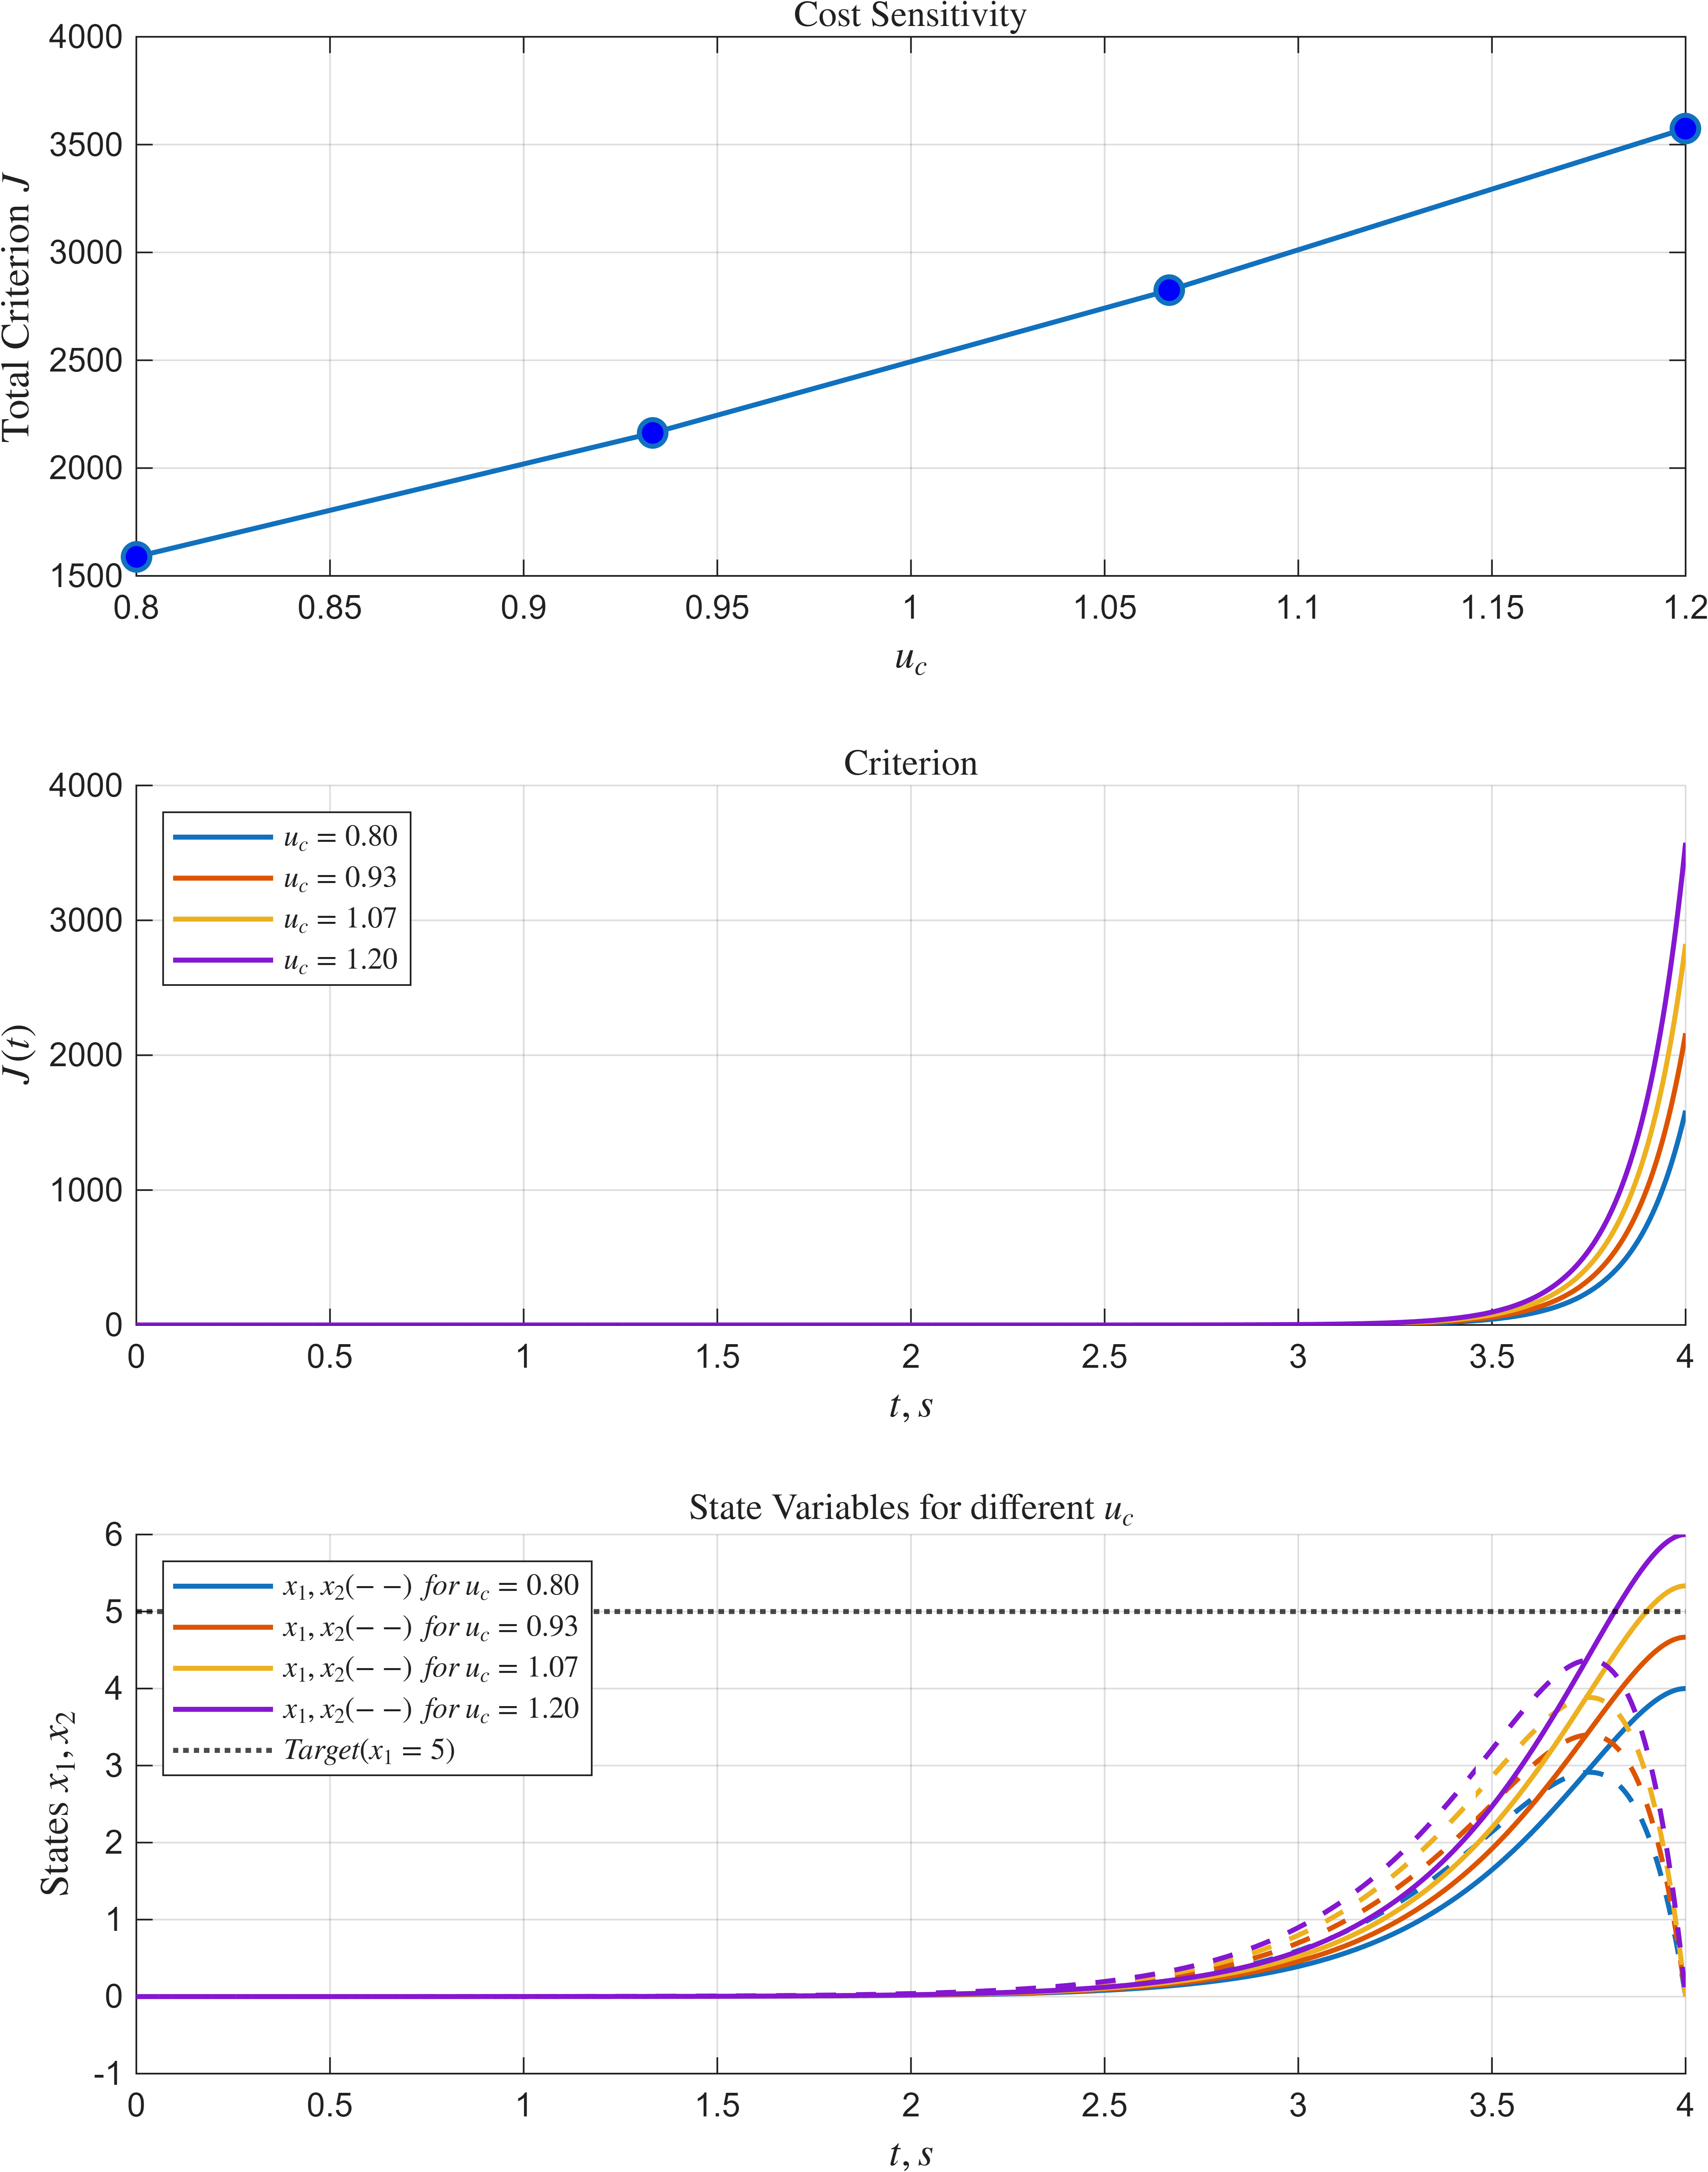
\includegraphics[width=\linewidth,height=0.78\textheight,keepaspectratio]{lab1_plots2.png}
    \caption{Влияние множителя $u_c$ на критерий качества и траектории состояния}
    \label{fig:control-sensitivity}
\end{figure}

\clearpage
\section{Выводы}

С помощью принципа максимума получена краевая задача
для состояния объекта и сопряжённых переменных. Её аналитическое
решение позволило определить программное управление,
переводящее объект из $\bm x(0)=(0,0)^{\mathsf T}$
в $\bm x(4)=(5,0)^{\mathsf T}$. Строгая выпуклость критерия
при линейных ограничениях гарантирует единственность
и глобальную оптимальность найденного решения.

Моделирование подтверждает выполнение конечных условий;
полученное значение критерия составляет $J^*\approx2482{,}50$.
Изменение общего множителя управления на $\pm20\%$ приводит
к отклонению $x_1(4)$ на $\pm1$ от заданного значения.
Критерий изменяется пропорционально $u_c^2$.
Уменьшение критерия при ослаблении управления сопровождается
недостижением цели и не даёт более выгодного допустимого
решения исходной задачи.
